\documentclass[man, floatsintext]{apa7}

\usepackage{lipsum}
\usepackage{tabularray}
\usepackage{multirow}
\usepackage[american]{babel}

\usepackage{csquotes}
\usepackage[style=apa,backend=biber,doi=false,url=false]{biblatex}
\addbibresource{bibliography.bib}
\usepackage{float}
\usepackage{graphicx}
\graphicspath{{./figures}}
\title{Modelling the effects of information gathering on social decision making}
\shorttitle{Modelling the effects of information gathering on social decision making}

\author{Damon Hayhurst}
\date{\today}

\makeatletter
\renewcommand{\maketitle}{
	\begin{titlepage}
		\centering
		\vspace*{0.4in}
		{\Huge \bfseries \@title \par}
		\vspace{0.2in}
		{\LARGE Damon Hayhurst \par}
		\vspace{0.3in}
		{\Large Project Report Submitted as\par}
		{\Large partial fulfilment for the\par}
		{\Large Degree of Cognition and Computation,\par}
		\vfill
		{\Large Birkbeck, University of London\par}
		{\Large \@date \par}
		\vfill
		{\Large
			\begin{center}
				I confirm that this write up is my own work and does not involve\par
				plagiarism as defined in the module information provided
			\end{center}
		}
		{\Large Signed and dated\par}
		\vspace{1in}
	\end{titlepage}
}
\makeatother

% Custom abstract environment to center the text
\renewenvironment{abstract}{
	\clearpage
	\null
	\vspace*{0.4in}
	\begin{center}
		This is the abstract
	\end{center}
	
	\vfill\null
	\clearpage
}

\begin{document}

\maketitle

% Project execution which includes: originality of ideas, independence, ability to act on advice and time and effort expended

\abstract

% Abstract which includes: completeness, clarity and succinctness

\section{Introduction}

% Introduction which includes: breadth of the review, understanding of the literature, description of aims or hypotheses, organization and structure and clarity

% What is the breadth of the review?
% The review is about investigating the strategies employed when making decisions in a social context, using the messenger game as a framework within which to investigate such strategies. The breadth therefore comes from looking at investigations into the ways in which search strategies have been shown to influence decison making.
% Intertemporal Choice
% link between strategy and choice
% Bounded reality
% Process Tracing


%The background to the study should be provided here including a review of relevant literature and theory and clear statements about the aims and objectives of the study.

The aims of this study is to gain an insight into how the effects of information gathering influence our decision making in a social context.  Using process tracing, we hope to observe and characterise strategies that are used in order to arrive at these decisions. Such an approach hopes to shed light further on the processes that underlie decision making in human behaviour.


\subsection{Aims/Objectives}

\begin{itemize}
	\item Ask whether information gathering strategy can be used a predictor in social decision making
	\item Understand whether perceived monetary outcomes to self and another have an affect on the way we gather information
	\item Determine if information gathering strategy in social decision making reflects an individual preference
\end{itemize}

\subsection{Bounded Rationality}

Herbert A Simon first outlined the idea that human behaviour in decision making was not to be defined by the decisions taken but that of the information surrounding the decision. This concept of 'Bounded Rationality' suggested an approach that took consideration of the contextual information regarding the decision as well as the computational capacities available to the decision maker. The concept sought to defy prior notions that human behaviour in decision making could be understood through a global notion of homo economius; Where decisions taken by agents were always perfectly rational, seeking to maximise their own self interests, and, instead, suggested that a human's capability to be perfectly rational was constrained by internal and external constraints.

The approach proposed by Simon places as much of an emphasis on the processing of information during the decision making as the decision itself. Pivotal to the concept of 'Bounded Rationality', Simon suggested that human's mental capacity to make choices is subject to heuristics or mental simplifications that contend with it's ability to be a perfectly rational agent but aid it's ability to make decisions in the face of increasing complexity (\cite{payneTaskComplexityContingent1976}).  Simon outlined Satisficing as a key mechanism  employed in the face of decisional complexity. Such a model of process attempts to define the appropriate option amongst choices as being the first option to surpass pre conceived threshhold. Rather than cope with the cognitive overhead of comparing every option against all of the others in a perfectly{MouselabWEBa} rational manner, humans will opt for the first choice that is deemed sufficient and satisfactory (\cite{simonRationalChoiceStructure1956d}, \citeyear{simonBehavioralModelRational1955}).

Early work into the mechanisms that perpetrate Simon's notion of constrained rational behaviour in human's uncovered the necessity for capturing process data. A model that was developed prior to this notion was the Priority Heuristic. The Priority Heuristic attempted to explain choices within the context of simple monetary gambles using an ordered list of criteria. While the mechanism was shown to be significant at the aggregate level, the model failed to capture differences at the individual level. Further research into the manifestation of the Priority Heuristic, using process data, uncovered that in actual fact the underlying process did not mimic the priority ordering set out by the heuristic. The data, however, revealed that choice could be predicted significantly by the number of transitions into and out of a choice. The uncovering of such mechanisms highlights the need for processing data in explaining how humans make decisions. Process data can provide the explanatory power for decision making differences and inform the development of heuristics that can be applied at the individual level ((\cite{brandstatterPriorityHeuristicMaking2006}, (\cite{willemsenVisitingDecisionFactory2011})).

%It is important to note that it is widely believed that human's decision making strategy is constructed contingent on the task demands and individual preferences. Decision making strategies have been shown to vary widely based on the number of choices at hand and the task complexity (\cite{payneWalkingScarecrowInformation2004}). Human's have a 'toolbox' of strategies which can be utilised in the cwhen it comes to information gathering and the choice reflects task demands and individual preferences. Such strat

\subsection{Process Tracing}

Process Tracing is the application or methodology within which attempts to gain insight into the decision making process through the extraction of data from specialised equipment. Methods vary from the simple writing of thoughts spoken out loud by the participant to the more involved methods that include neural tracing in an MRI machine. Such instrumentation hopes to extract a level of the data from the decision making process and the representation of the information within it in to further inform the development of process models.

\subsubsection{MouseLabWeb}

MouseLabWeb is one such development in process tracing that fosters an environment fit for observing the information gathering stage in decision making. Utilising the dynamic properties of javascript in the context of a web page, MouseLabWeb describes a framework within which information, important to the decision at hand, is hidden from view. Only to be uncovered, by hovering over the panels with a mouse cursor does the information reveal. The mouse cursor movements are tracked and then stored on a trial by trial basis. Such data can be used to observe how we deliberate between two options that are hidden from view and how much we dwell on each particular bit of infomation. By capturing this information alongside the chosen outcome, a representation of the decision making process can be built (\cite{MouselabWEBa}).



% paragraph on contingency



\subsubsection{MouselabWeb}

\subsection{Intertemporal Choice task}

\subsection{Social Decision Making}


\section{Methods}

% Methods which includes: completeness, justification of choices/decisions made, organization and structure, clarity, reference to ethics

% This section is composed of several sub-sections and should give sufficient information to enable the reader to know exactly what was done:
%
%Participants (in projects using human participants).This will be skipped if you are not using human participants. Please specify in this section that ethical approval was obtained and include the ethics approval number and the title of the ethics application.
%
%Materials and Stimuli (all stimuli involved in your project, including software, questionnaires, programmes, interview schedules, for example). Feel free to include pictures of your stimuli. Describe everything.
%
%Design and Procedure (this section should be detailed enough that someone not familiar with your project should be able to run it themselves/understand how you recruited participants, collected data and so on). 

A variation of the Message game was used in the experiment. The game uses honesty to illustrate how decision making can be affected by value judgements that pit our own self interest against our altruistic sensitivities. The game involves two roles. The Sender and the Receiver. The Sender must send a message to the Receiver informing them of a particular box to open from a choice of four. Each of the boxes contains differing amounts of money for the Sender and the Receiver should that box be opened. The Sender can ultimately see what's inside each of the boxes in terms of how much money they will receive versus the amount that the Receiver will. Only the Receiver opens the box, however. A message is sent by the Sender to the Receiver with words to the affect of 'Box X is best for you'. The dishonesty comes from the Sender being able to suggest a box that might not necessarily represent the truth and instead picking a box that contains a larger amount of money for themselves and less money for the Receiver than that of one of the other boxes.With the Receiver unable to see the quantity of money they potentially missed and in this variation, two of the boxes being blank, the Receiver has no choice but to trust the potentially dishonest disclosed by the Sender.

The experiment took place through a web browser. Each participant was provided with a run through of the game from the perspectives of both roles. Showing the nature of choosing a box to suggest as the Sender and opening a suggested box as the Receiver. With an learned understanding of both roles, the rest of the experiment takes place with the participant in the Sender role. Over 80 trials, differing values are placed in to two of the four boxes within the screen's width. The position of the two boxes that contain values varies as do the values contained within each of them. Each box has two values inside containing the listed values received for both the Sender and the Receiver. Each of these values is covered up and in order for the participant (or Sender) to view the value, they must hover over each item in order to see the contained value. Being unable to see the values without hovering over them suggests that when a participant is hovering over a value there is suggestion that they are dwelling on such an idea.

% OVer experiement was found no difference mouse vs vision
% Look into the idea of dwelling on something by looking at it.

\subsection{Processing the data}

\subsubsection{Preprocessing}

All analyses was performed on participants that matched the condition wherein a proportion of their responses represented choices that were lying to the receiver. Participants who selected over 95\% lie choices were not considered and similarly participants who chose over 95\% truthful options were not selected either. Any participant who picked one of the two blank boxes in over 5\% trials were also not selected. Any participant who did not finish the 80 trials was also removed from the analyses suggesting a lack of engagement. Similarly, any trials that 

\subsubsection{Identifying areas of interest}

\subsubsection{Creating a timeline}

\subsection{Average analysis}

\subsection{Distance analysis}

\subsubsection{Creating time series sequences}

\subsubsection{Measuring the distance between trials}

\subsubsection{Clustering}


\section{Results/Findings}

\subsection{Trial and Participant Quantities}

The processing of data removed a proportion based on criteria that represented a lack of engagement with the experiment. six participants were removed for not finishing it. 20 were removed for telling the truth over 95\% the time and a further 14 participants were removed for recommending the blank boxes to the receiver in over five percent of the trials.  Interestingly, no participants were removed for lying over 95\% of the time; despite this being the approach favoured in game theory.  A further 40 trials were removed from the dataset because they recorded decision making times that were three standard deviations away from the mean. An approach also taken by \citeauthor{reeckSearchPredictsChanges2017b}, suggesting a similar lack of engagement with the task at hand.

Irregularities and missing data that represented a failure in process tracing were also removed from the dataset. 10 participants were removed for having not recorded mouse coordinates in over 85\% of their trials and a further 108 trials removed from the remaining valid set because of similar lack of mouse coordinates. Irregularities in some of the coordinate data meant that AOIs could not identified through measurement. 42 trials were removed because of this and one participant also, that failed to record screen width data. If such impairments in the dataset had been included by merely estimating their missing qualities, it would have compromised the overall integrity. Omitting them highlights the essential role of accurate process tracing.

After accounting for engagement criteria and irregularities, the number of valid trials was recorded for each participant and a further two participants were excluded from the analysis. The number of valid trials for each of these participants represented a quantity that was less than three quarters of the intended 80 trials for each participant. Given, the ordering of each trial was randomised, the set of valid trials for each of these participants could represent biases in likelihood to lie relative to the whole data set.

From the original pool of 89 participants, only 36 remained after all removals. An overall data set that contained 2783 trial instances each with a valid process trace.

\begin{figure}[H]
	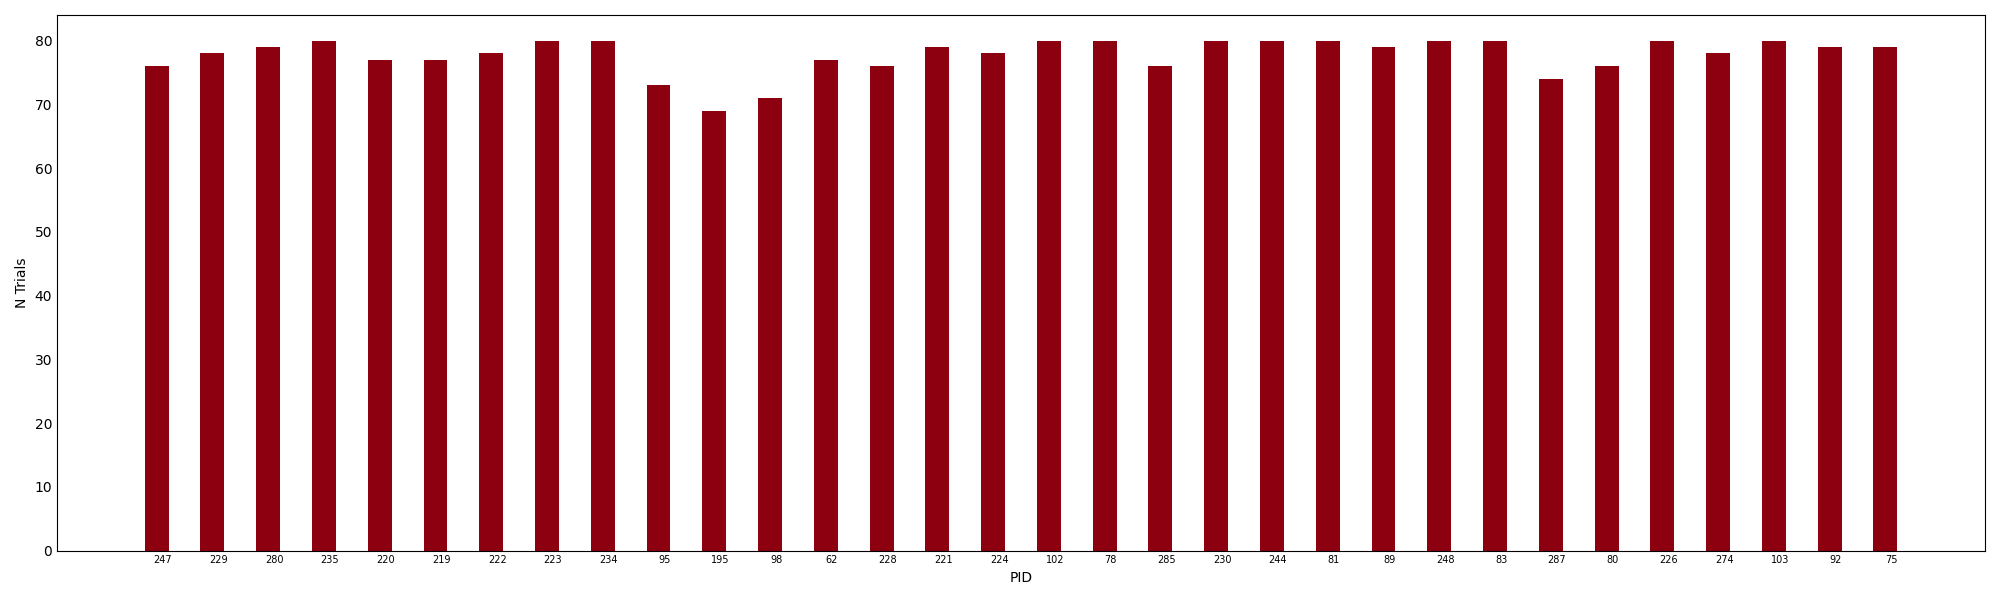
\includegraphics[width=\linewidth]{../plots/RESPONSE/NTrialsByPID.png}
	%\figurenote{This is a great figure.}
	\label{fig:NTrialsByPID}
	\caption{Bar graph representing number of trials in the final valid data set for each participant.}
\end{figure}

\subsection{Descriptives}

\subsubsection{Lie Percentage}

Across trials the propensity to lie displayed a high degree of variance. The average likelihood to lie on any given trial was 39\% $(SD = 49\%)$. Across participants, the propensity to lie was measured between 3\%-91\% for a given individual. Across instances of unique trial, where unique is defined by the specific quantities pertained to in the boxes, the range was 0-87\% for any given trial.

\begin{figure}[H]
	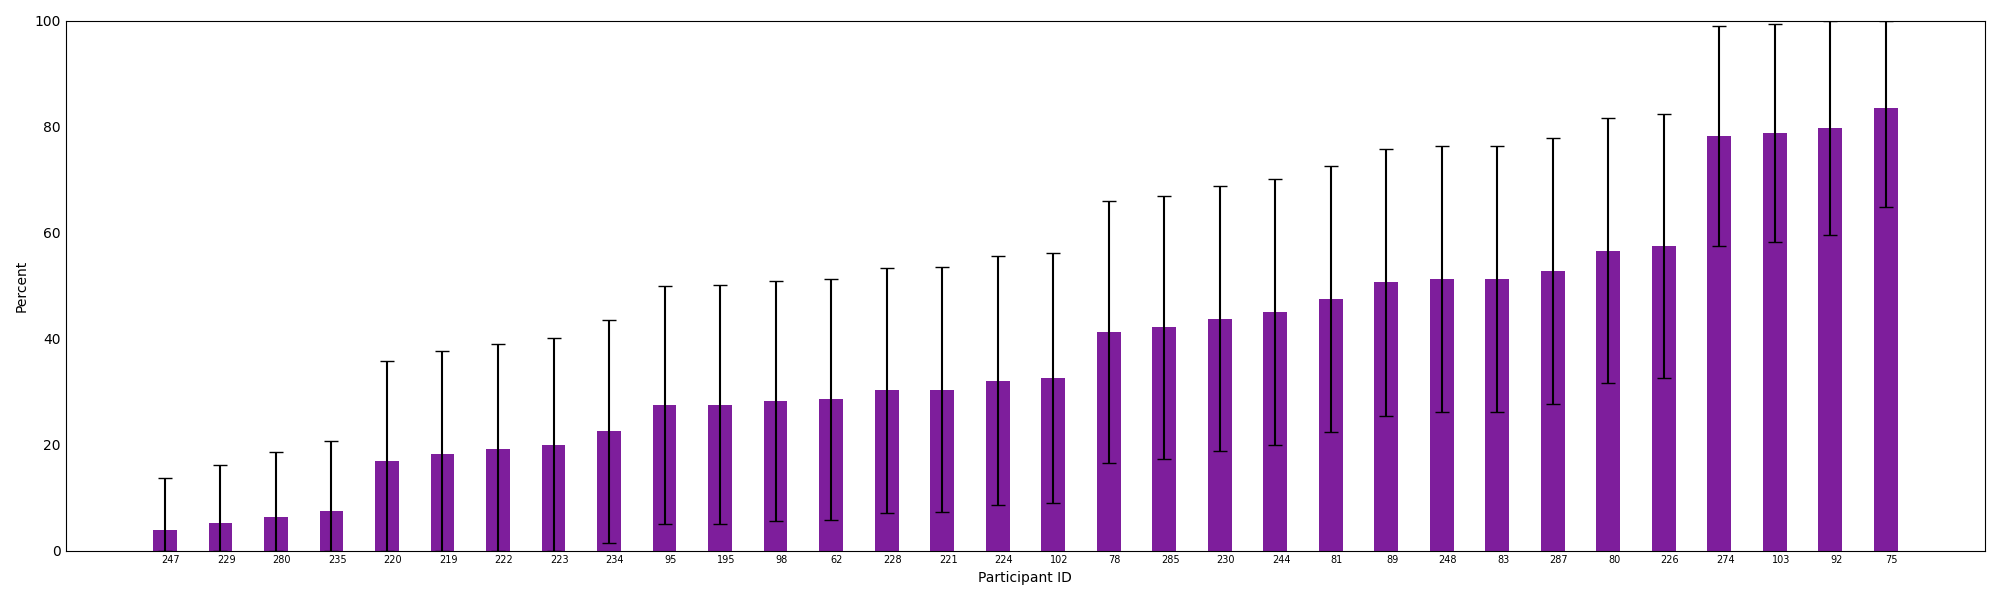
\includegraphics[width=\linewidth]{../plots/RESPONSE/PIDPercentLiesPlot.png}
	%\figurenote{This is a great figure.}
	\label{fig:PIDPercentLiesPlot}
	\caption{Bar graph representing the percentage amount of lies across participants}
\end{figure}

\begin{figure}[H]
	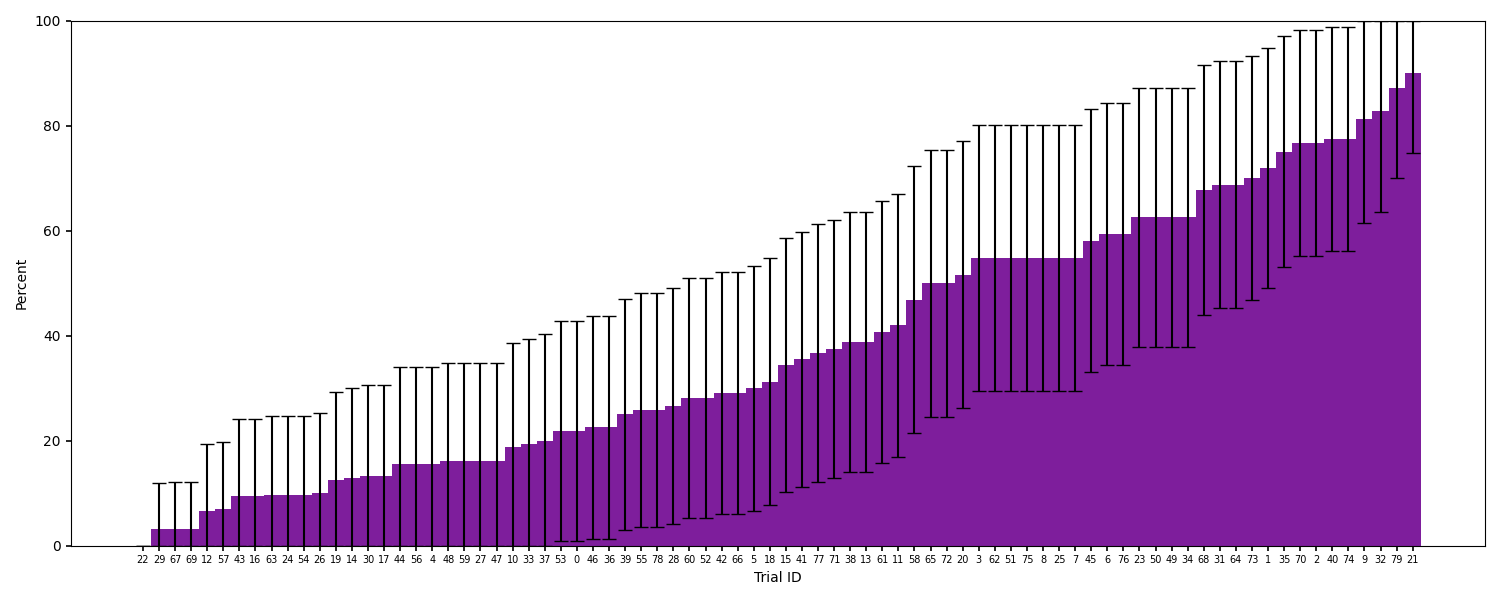
\includegraphics[width=\linewidth]{../plots/RESPONSE/TRIALIDPercentLies.png}
	%\figurenote{This is a great figure.}
	\label{fig:TRIALIDPercentLies}
	\caption{Bar graph showing the percentage of lies for each trial condition.}
\end{figure}

\subsubsection{Dwell Time Distribution}

Reaction time (or the time it takes to make a decision) showed a large amount of range. The average reaction time was 6324 ms $(SD = 3059$ms$)$ and ranged from 2114ms - 22333ms,

\begin{figure}[H]
	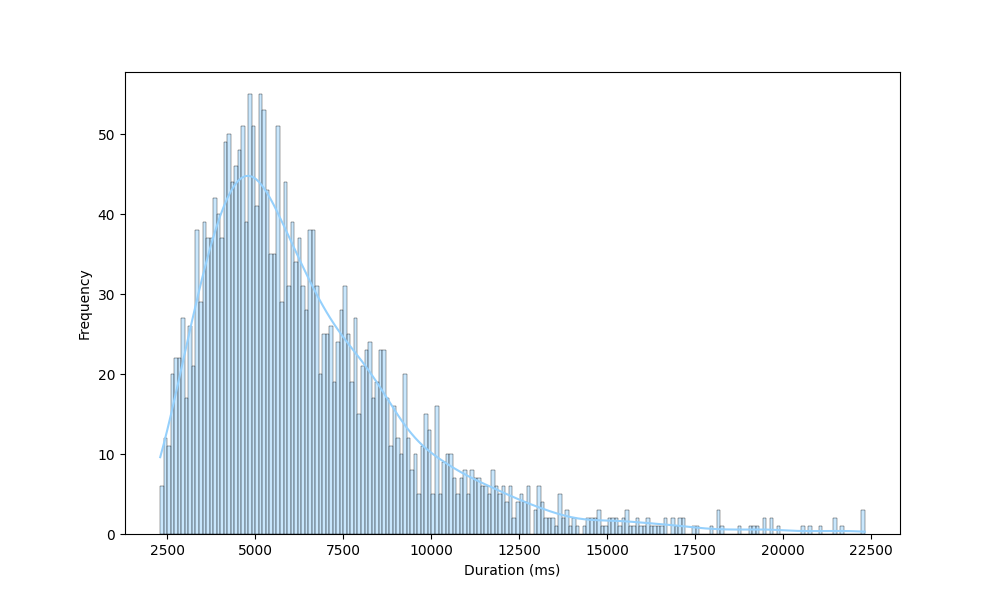
\includegraphics[width=\linewidth]{../plots/Dwell/RTDistPlot.png}
	%\figurenote{This is a great figure.}
	\label{fig:RTDistPlot}
	\caption{Distribution of reaction time ie. time taken to make a decision.}
\end{figure}

The amount of spent dwelling on one of the four AOIs on the screen was considered. Values ranged from 4ms - 7082ms. The AOIs, SELF LIE ($M = 381$ms, $SD = 382$ms), SELF LIE ($M = 350$ms, $SD = 328$ms), OTHER LIE ($M = 455$ms, $SD = 411$ms) and OTHER TRUTH ($M = 477$ms, $SD = 416$ms) all recorded means within 100ms of one another. A large proportion of the trials reported no dwell time for at least one of the given AOIs. Both SELF TRUE and SELF LIE  were absent from the dwell timelines of 477 and 464 trials respectively, representing an omission rate of almost 20\%. OTHER TRUE and OTHER LIE were omitted from 218 and 220 respectively representing just under 10\% of all trials.

\begin{figure}[H]
	\caption{Distribution of average dwell time for each AOI. The distribution only accounts for average dwell time of each AOI that was under 1000ms. Each AOI also had a proportion of average dwell times that were 0, which were also omitted.}
	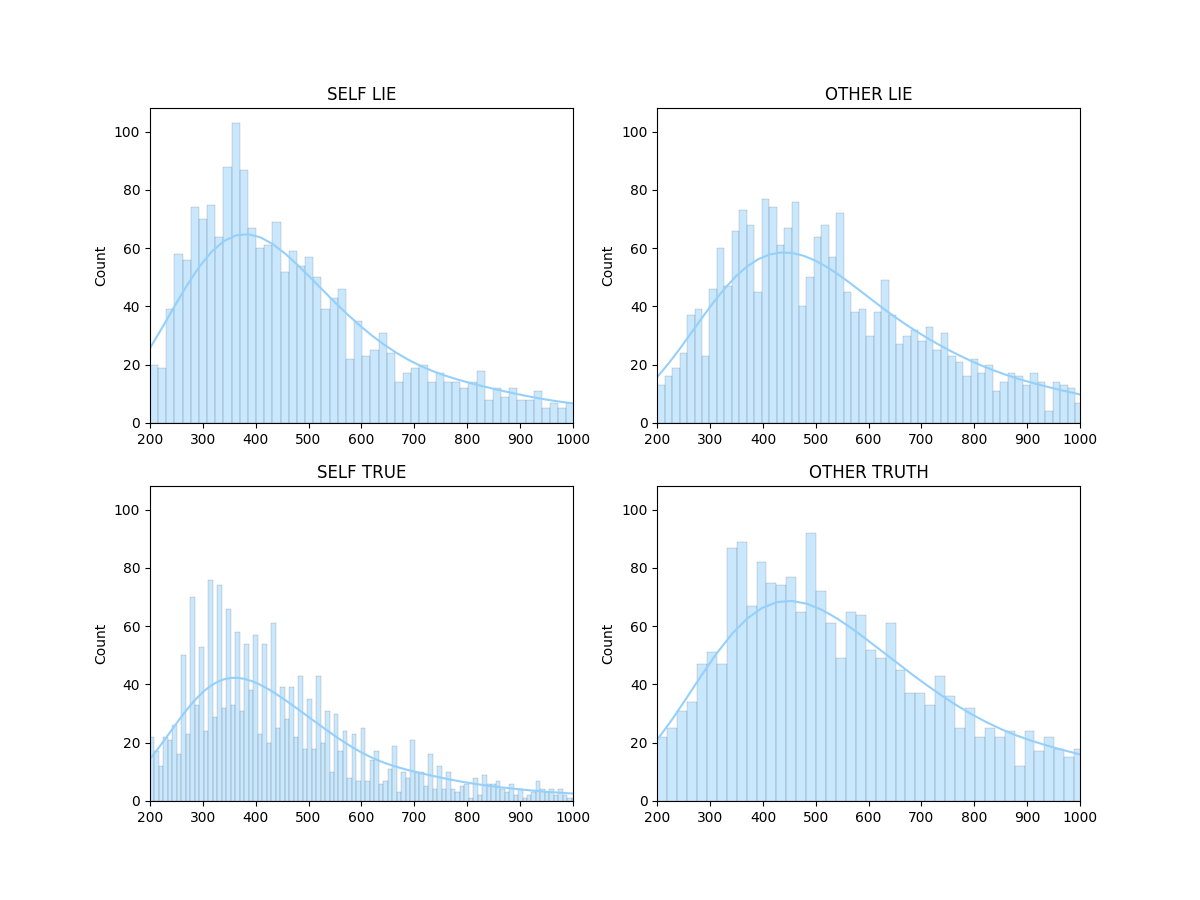
\includegraphics[width=\linewidth]{../plots/Dwell/DwellDistPlot.png}
	%\figurenote{This is a great figure.}
	\label{fig:DwellDistPlot}
\end{figure}


\begin{figure}[H]
	\caption{Distribution of number of transitions between AOIs across trials.}
	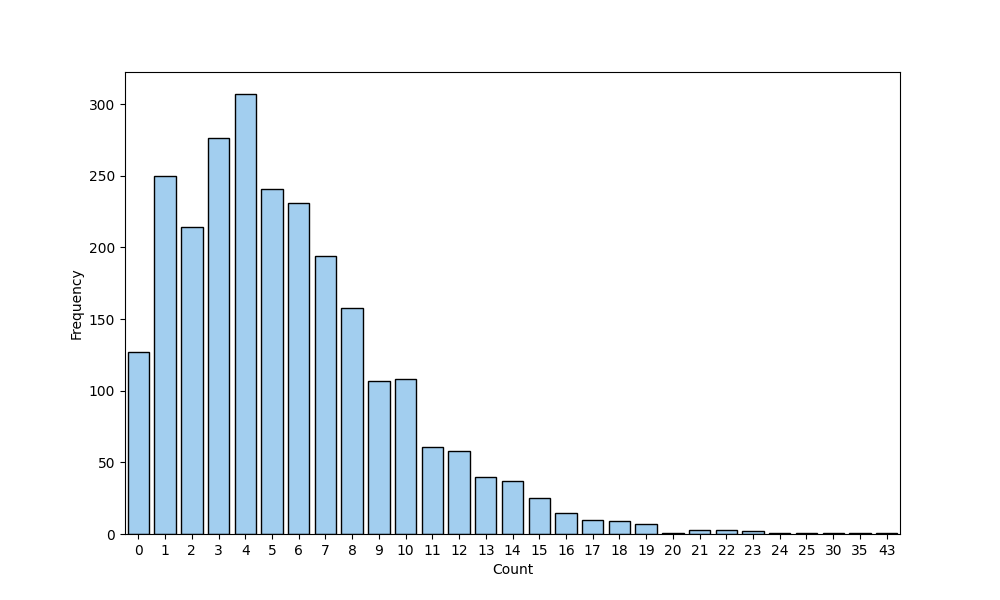
\includegraphics[width=\linewidth]{../plots/Dwell/N_TransitionsDistPlot.png}
	%\figurenote{This is a great figure.}
	\label{fig:NTransitionsDistPlot}
\end{figure}

The number of transitions where a participant would move the cursor from one AOI to another was also observed. The mean number of transitions between AOIs was ($M = 455$ms, $SD = 411$ms).


\subsection{Task Analysis}

\subsubsection{Lie Percentage}

Each of the trials involved giving differing amounts to the sender and the receiver based on whether the sender decided to lie or not. The average net gain to the sender was 12 $(SD = 13)$ per trial. The median was 8 and had an interquartile range of 4 (Q1) - 17 (Q3). The average loss to the receiver was 11 $(SD = 9)$ with a median of 8 and an interquartile range of 4 (Q1) - 15 (Q3).

\begin{figure}[H]
	\caption{Bar chart showing the amount gained by the sender should they choose to lie in the corresponding trial.}
	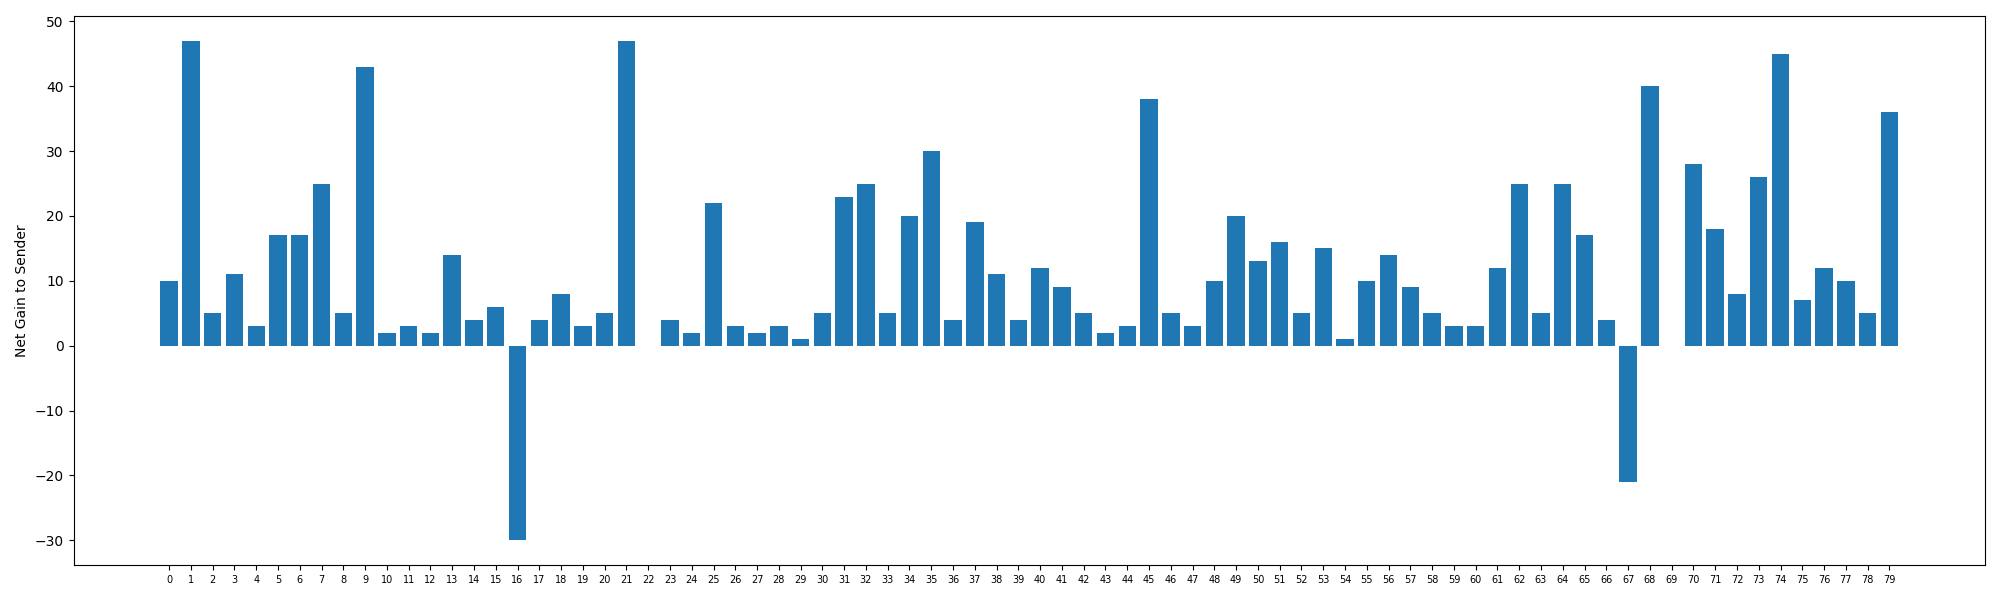
\includegraphics[width=\linewidth]{../plots/TrialIndex/Gains.png}
	%\figurenote{This is a great figure.}
	\label{fig:Gains}
\end{figure}

The percentage of senders that chose to lie in the experiment increased as the net gain to the sender did.  Senders lied the least when they incurred a net loss by lying $(M = 6\%$, $SD = 23\%)$. From net gains below 10 $(M = 26\%$, $SD = 44\%)$ to above 10 $(M = 55\%$, $SD = 50\%)$, the percentage who chose to lie increased. When gains were above 20 $(M = 68\%$, $SD = 46\%)$ and above 30 $(M = 73\%$, $SD = 44\%)$, the amount who decided to lie showed further increase but to a lesser extent.

\begin{figure}[H]
	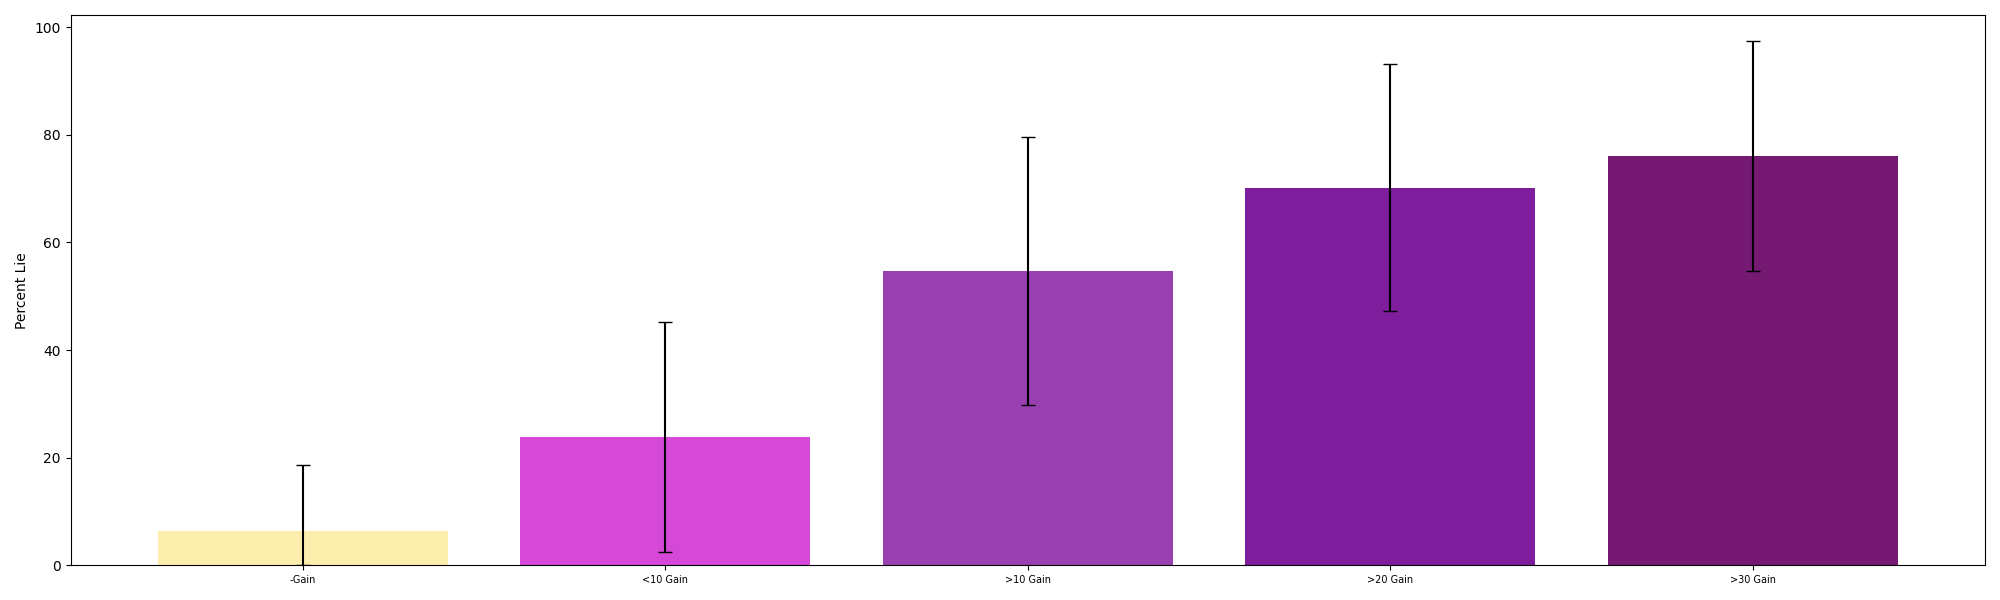
\includegraphics[width=\linewidth]{../plots/RESPONSE/NetGainLie.png}
	\caption{Percentage who chose to lie based on the amount gained by lying.}
%	\figurenote{+10 gain represents the proportion who chose to lie for all amounts above 10 and also applies for +20 and +30.}
	\label{fig:NetGainLie}
\end{figure}

A significant difference in the proportion of lies was observed across trials where the sender gained less than 10 and when they received more than 10, $\chi^2(1,$ $N=2783) = 231,$ $p=.001$. A significant difference was also noticed in trials where the sender received more than and less than 30 $\chi^2(1,$ $N=2783) = 145,$ $p<.001$.

\begin{figure}[H]
	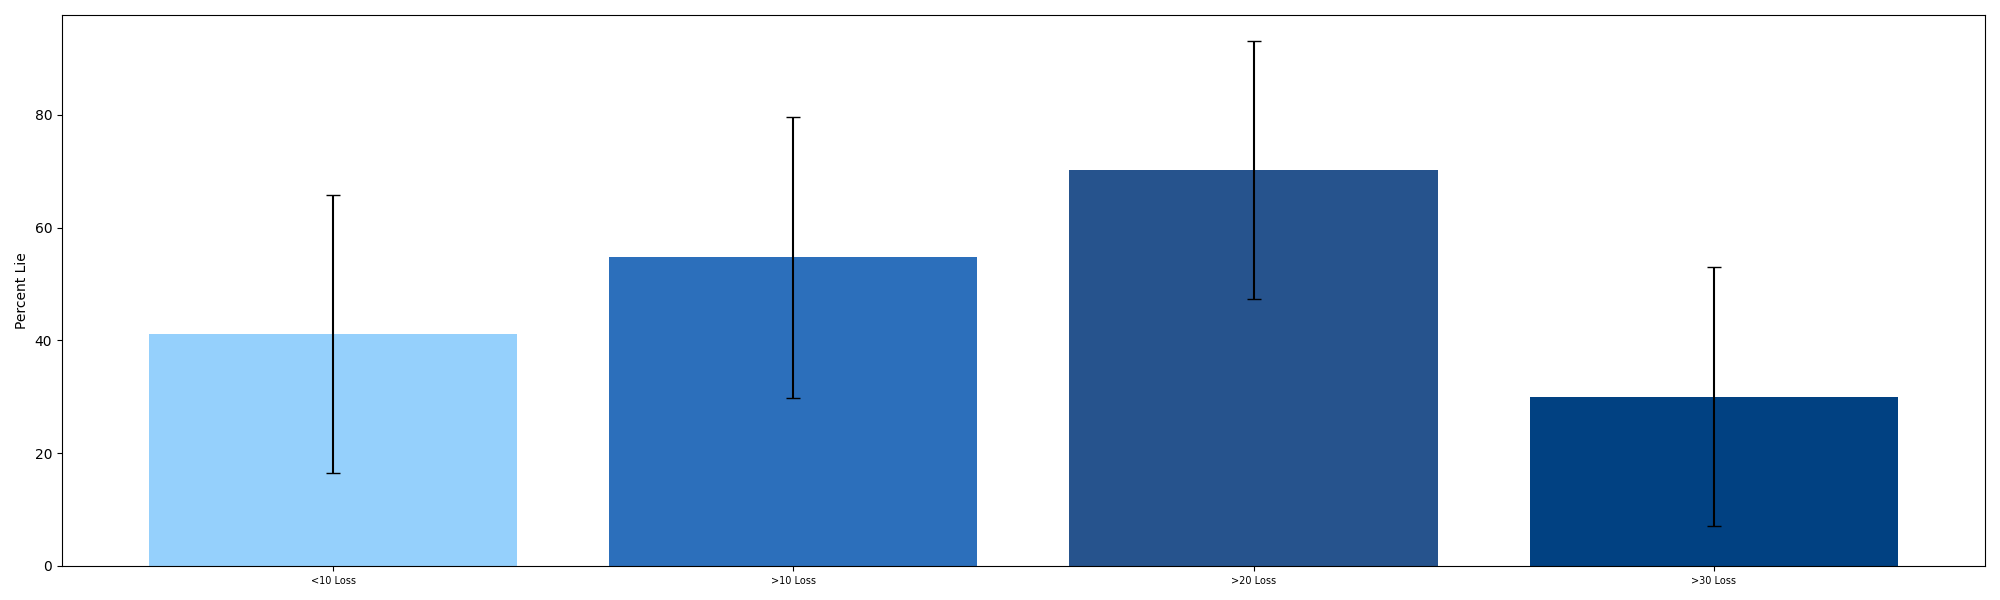
\includegraphics[width=\linewidth]{../plots/RESPONSE/NetLossLie.png}
	\caption{Percentage of senders who chose to lie based on how much the receiver would lose.}
%	\figurenote{+10 gain represents the proportion who chose to lie for all amounts above 10 and also applies for +20 and +30.}
	\label{fig:NetLossLie}
\end{figure}

Senders were less likely to lie when the losses to the receiver were great. From losses under 10 $(M = 42\%$, $SD = 49\%)$, losses greater than 10 $(M = 55\%$, $SD = 50\%)$ through to losses greater than 20 $(M = 68\%$, $SD = 47\%)$ the percentage of senders who chose to lie showed a notable increase. When losses to the receiver were larger than thirty the amount of senders who lied showed a notable decrease $(M = 32\%$, $SD = 47\%)$. 

The difference in lie percentage between trials where losses to the receiver were over 10 and trials where losses to the receiver were under 10 was shown to be significant $\chi^2(1,$ $N=2783) = 11,$ $p=.001$. However, differences in lie percentage were shown to be non-significant in trials where losses to the receiver were over and under 30 $\chi^2(1,$ $N=2783) = 3.3,$ $p=0.71$.

\subsubsection{Dwell Time}

\begin{figure}[H]
	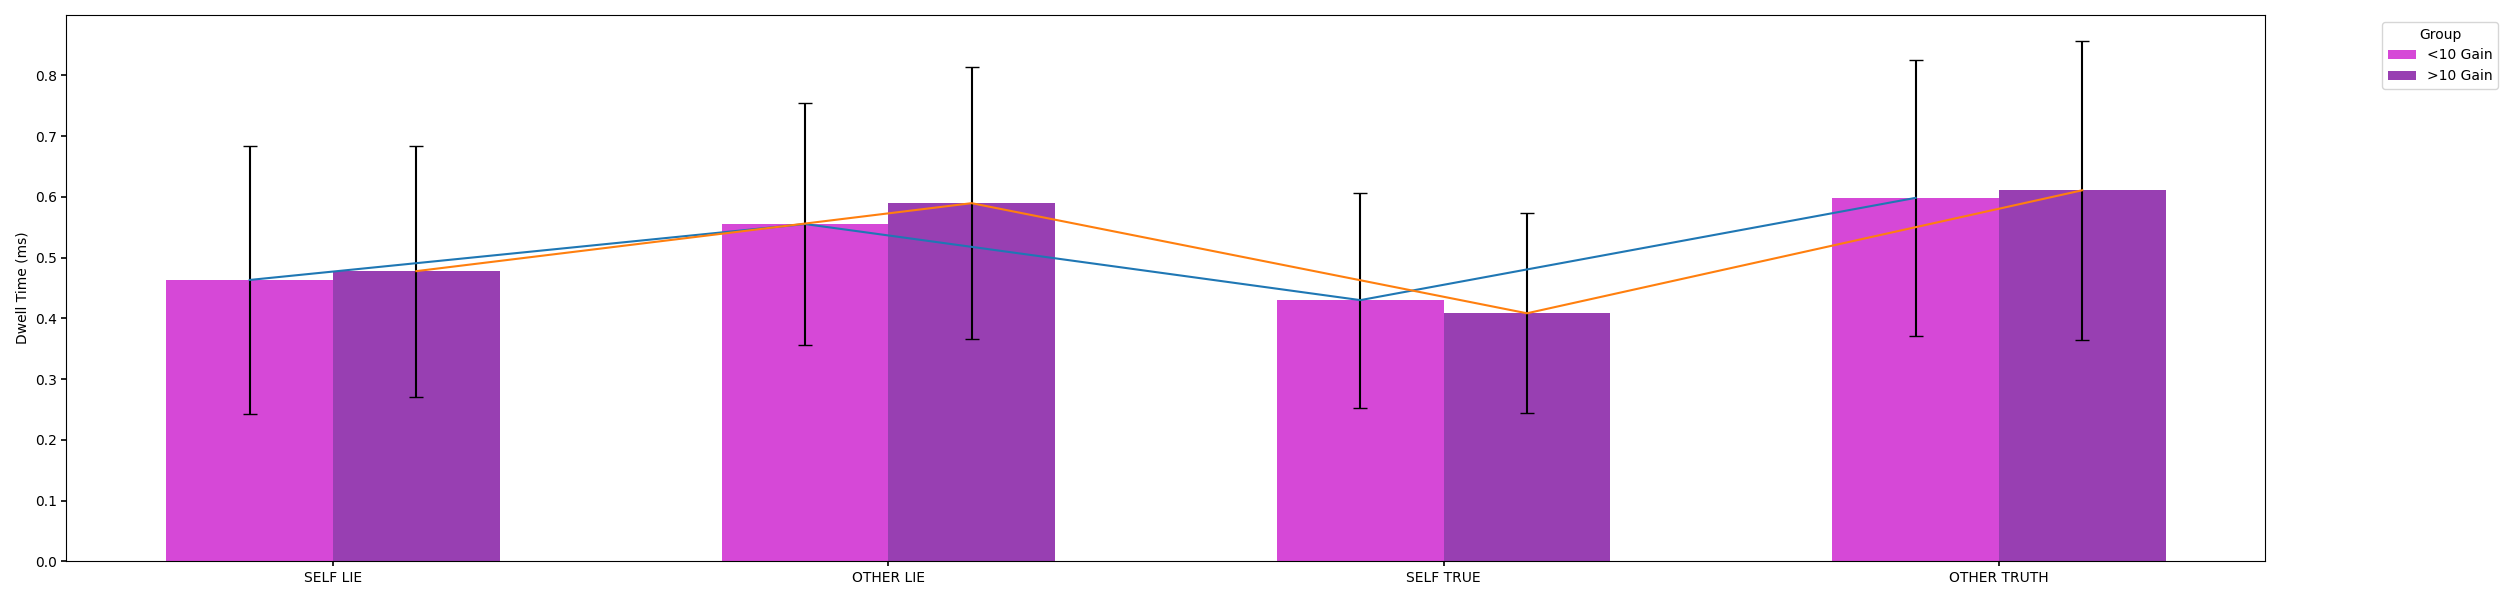
\includegraphics[width=\linewidth]{../plots/RESPONSE/AvgDwellPerGain.png}
	\caption{Average Dwell Time for each AOI comparison between trials where net gain to the Sender was less than 10 and trials where the net gain was more than 10}
	%	\figurenote{+10 gain represents the proportion who chose to lie for all amounts above 10 and also applies for +20 and +30.}
	\label{fig:AvgDwellPerGain}
\end{figure}

\begin{table}[H]
	\centering
	\begin{tabular}{|c|p{1.5cm}|p{2cm}|p{1.5cm}|p{2cm}|p{2cm}|p{1.5cm}|}
		\hline
		\multirow{2}{*}{} & \multicolumn{2}{c|}{<10 Gain to Sender} & \multicolumn{2}{c|}{>10 Gain to Sender} & \multicolumn{2}{c|}{T-test result} \\ \cline{2-7}
		& $M$ (ms) &$SD$ (ms) & $M$ (ms) & $SD$ (ms) & $t(2781)$ & $p$ \\ \hline
		SELF LIE& 0.38 & 0.40 & 0.38 & 0.36 & -0.26 & .793  \\ \hline
		SELF TRUE & 0.35 & 0.33 & 0.34 & 0.33 & -0.74 & .460  \\ \hline
		OTHER LIE & 0.45 & 0.39 & 0.47 & 0.44 & 1.3 & .390 \\ \hline
		OTHER TRUTH & 0.45 & 0.39 & 0.47 & 0.44& -0.50 & .622 \\ \hline
	\end{tabular}
	\vspace{0.3cm}
	\caption{Comparison of mean and standard deviation of dwell times for each AOI across trials where the net gain to Sender was less than 10 versus trials where the net gain was more than 10. (FDR Corrected)}
	\label{tab:NetGainDwell}
\end{table}

Table \ref{tab:NetGainDwell} shows that there was an no significant difference between the average dwell time of the four AOIs across trials where the net gain to the Sender was less than 10 versus when it was more than 10.

\begin{figure}[H]
	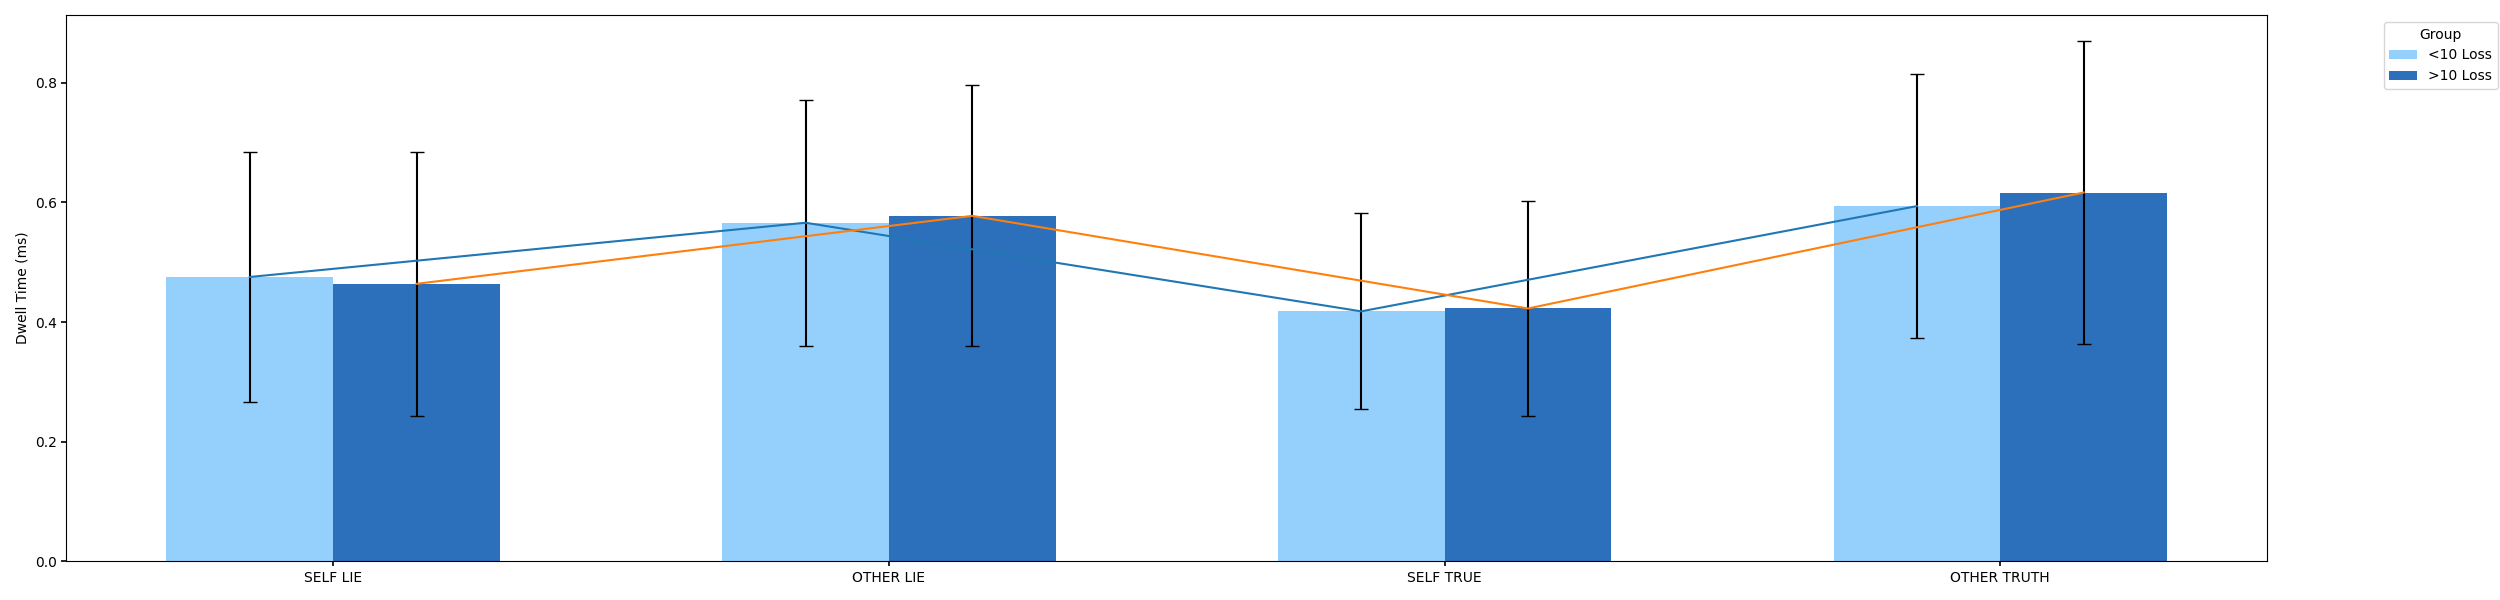
\includegraphics[width=\linewidth]{../plots/RESPONSE/AvgDwellPerLossPlot.png}
	\caption{Average Dwell Time for each AOI comparison between trials where net loss to the Receiver was less than 10 and trials where the net loss was more than 10}
	%	\figurenote{+10 gain represents the proportion who chose to lie for all amounts above 10 and also applies for +20 and +30.}
	\label{fig:AvgDwellPerLoss}
\end{figure}

\begin{table}[H]
	\centering
	\begin{tabular}{|c|p{1.5cm}|p{2cm}|p{1.5cm}|p{2cm}|p{2cm}|p{1.5cm}|}
		\hline
		\multirow{2}{*}{} & \multicolumn{2}{c|}{<10 Loss to Receiver} & \multicolumn{2}{c|}{>10 Loss to Receiver} & \multicolumn{2}{c|}{T-test result} \\ \cline{2-7}
		& $M$ (ms) &$SD$ (ms) & $M$ (ms) & $SD$ (ms) & $t(2781)$ & $p$ \\ \hline
		SELF LIE& 0.39 & 0.38 & 0.38 & 0.36 & -0.86 & .784  \\ \hline
		SELF TRUE & 0.34 & 0.30 & 0.34 & 0.39 & 1.2 & .459  \\ \hline
		OTHER LIE & 0.44 & 0.38 & 0.47 & 0.44 & 1.5 & .195 \\ \hline
		OTHER TRUTH & 0.47 & 0.40 & 0.47 & 0.42& 1.3& .387 \\ \hline
	\end{tabular}
	\vspace{0.3cm}
	\caption{Comparison of mean and standard deviation of dwell times for each AOI across trials where the net gain to Sender was less than 10 versus trials where the net gain was more than 10. (FDR Corrected)}
	\label{tab:NetLossDwell}
\end{table}

Similarly, in Table \ref{tab:NetLossDwell}, there was no significant difference between the dwell times in trials where the loss to the Receiver was above 10 versus trials where it was below 10.

\subsubsection{Number of Transitions}

\begin{figure}[H]
	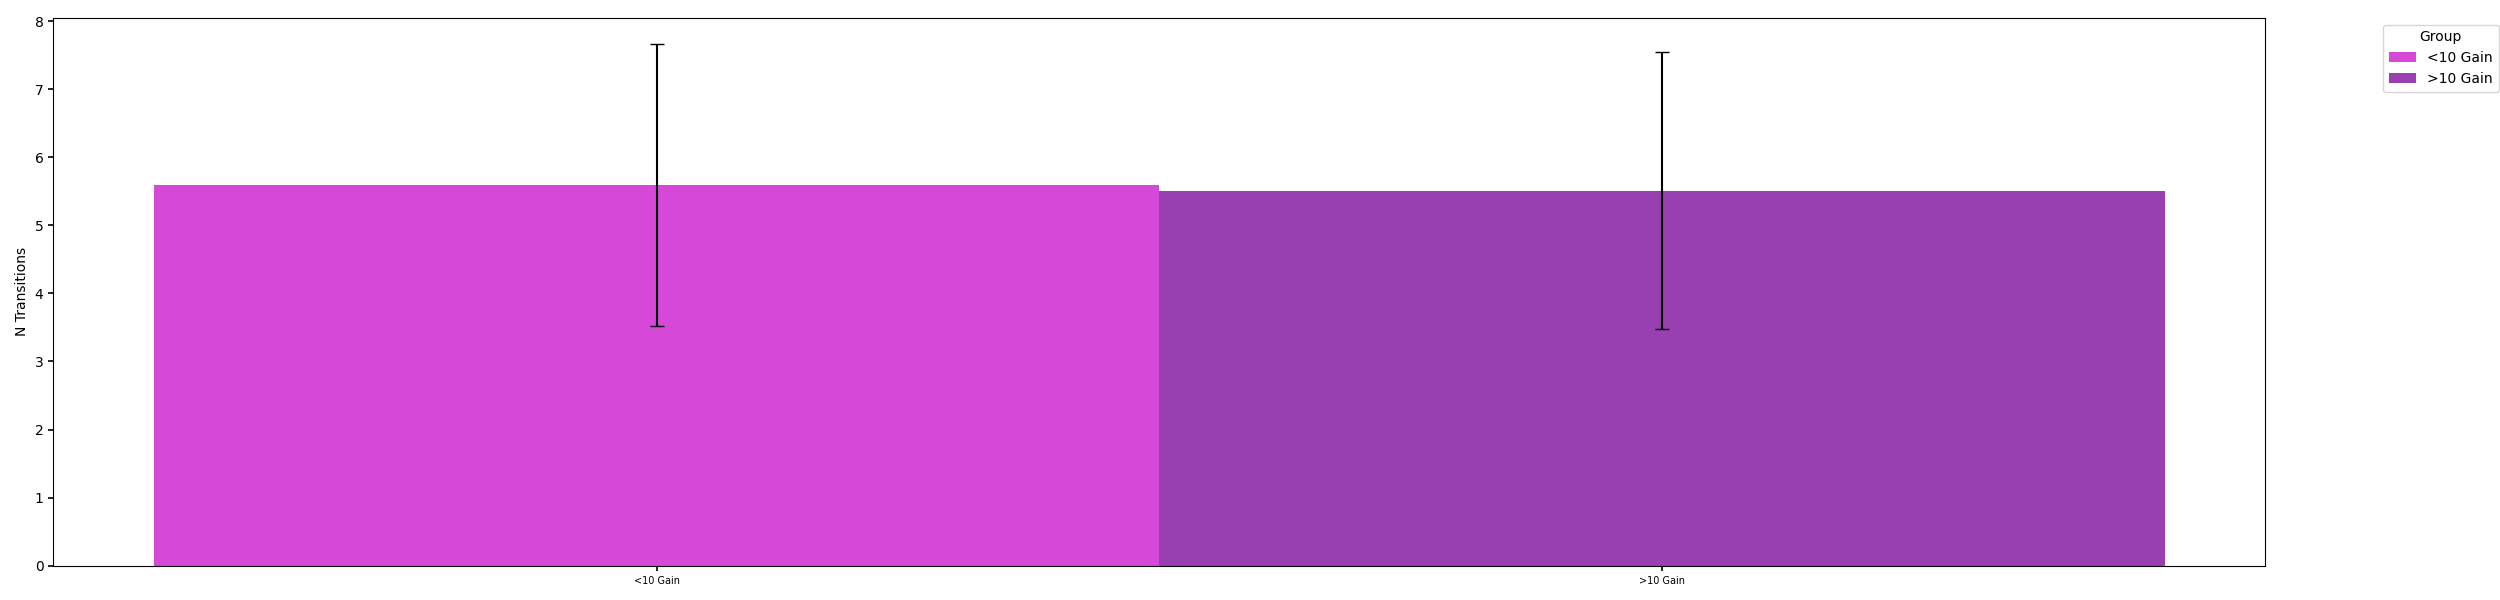
\includegraphics[width=\linewidth]{../plots/RESPONSE/NTransitionPerGain.png}
	\caption{Comparison of average number of transitions between trials where the net gain to the Sender was less than 10 and trials where the net gain was more than 10}
	%	\figurenote{+10 gain represents the proportion who chose to lie for all amounts above 10 and also applies for +20 and +30.}
	\label{fig:NTransitionPerGain}
\end{figure}

The difference in number of transitions proved not to be significant when comparing trials where the net gain to the Sender is above $(M = 42\%$, $SD = 49\%)$ or below 10 $(M = 42\%$, $SD = 49\%)$, $t(2781)=2.5$, $p=.001$.

\begin{figure}[H]
	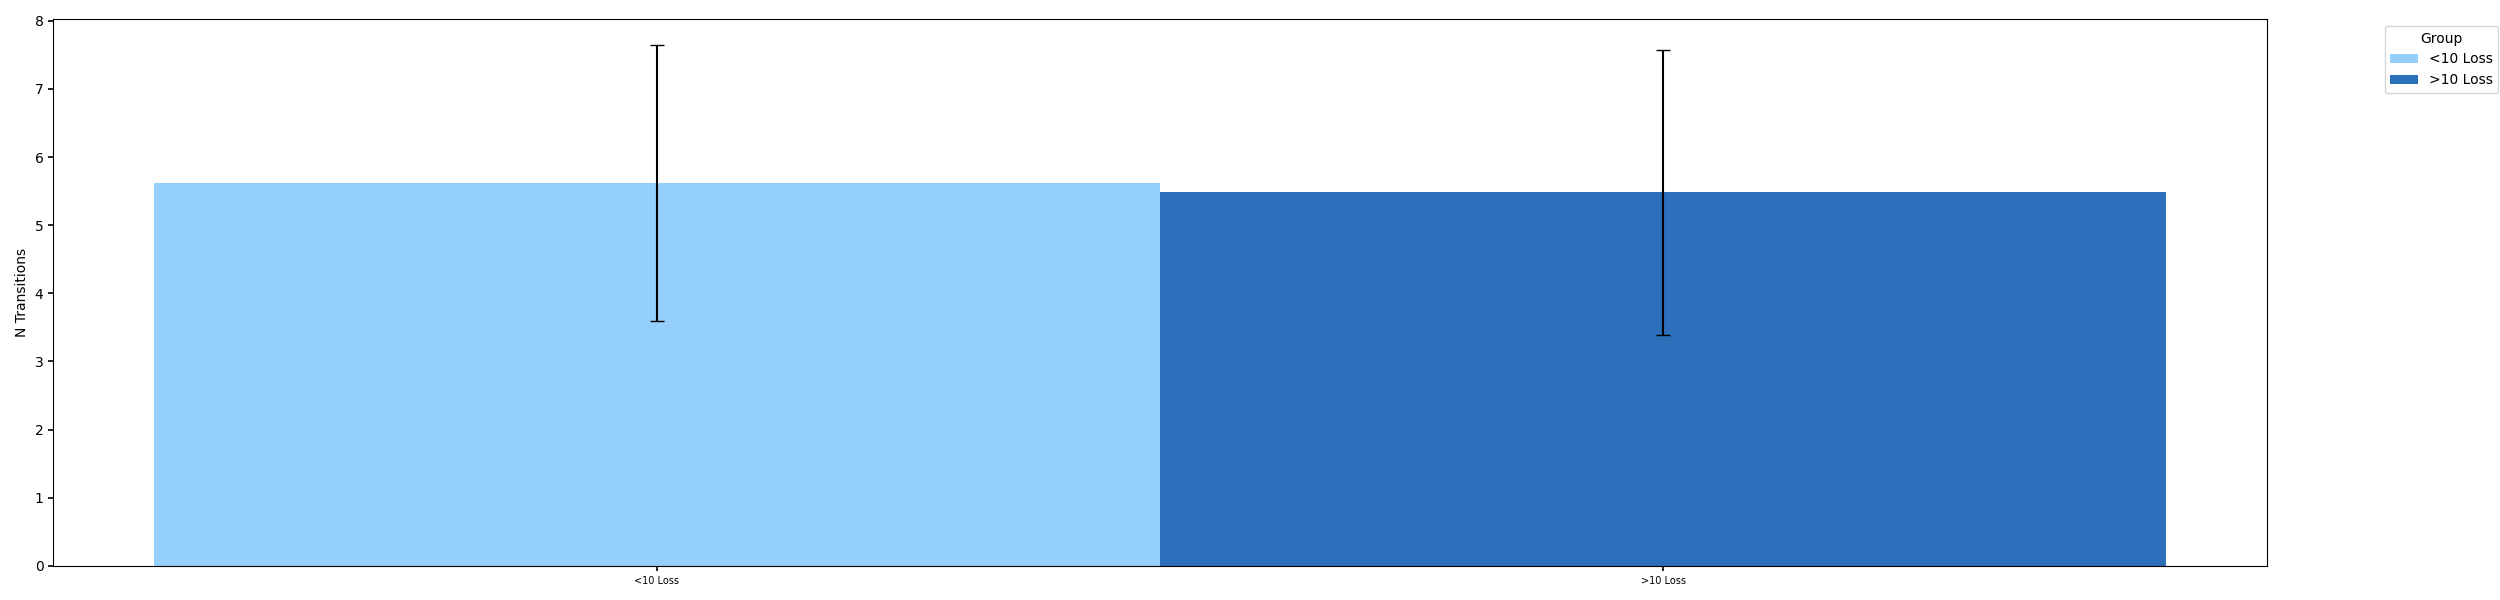
\includegraphics[width=\linewidth]{../plots/RESPONSE/NTransitionPerLossPlot.png}
	\caption{Comparison of average number of transitions between trials where net loss to the Receiver was less than 10 and trials where the net loss was more than 10}
	%	\figurenote{+10 gain represents the proportion who chose to lie for all amounts above 10 and also applies for +20 and +30.}
	\label{fig:NTransitionPerLoss}
\end{figure}

Similarly the difference in number of transitions showed to be insignificant when comparing trials where the Receiver made a loss of above $(M = 6.7\%$, $SD = 4.9\%)$  or below 10 $(M = 6.8\%$, $SD = 4.8\%)$ from lying, $t(2781)=-0.99$, $p=.648$.
% Results/Findings which includes: analyses performed, reporting of analyses, use of graphs/tables/diagrams, organization and structure, and clarity
% analyses performed:
% RT, Dwell Times
% Gains
% DTW 

\subsection{Participant Analysis}

An analysis was performed on the distance data extracted from the time series analysis at the participant level. The results of which, are taken from averaging the distance between all of the trials of a single participant against another. Through hierarchical clustering and silhouette analysis, the participants were separated in to two clusters.

\begin{figure}[H]
	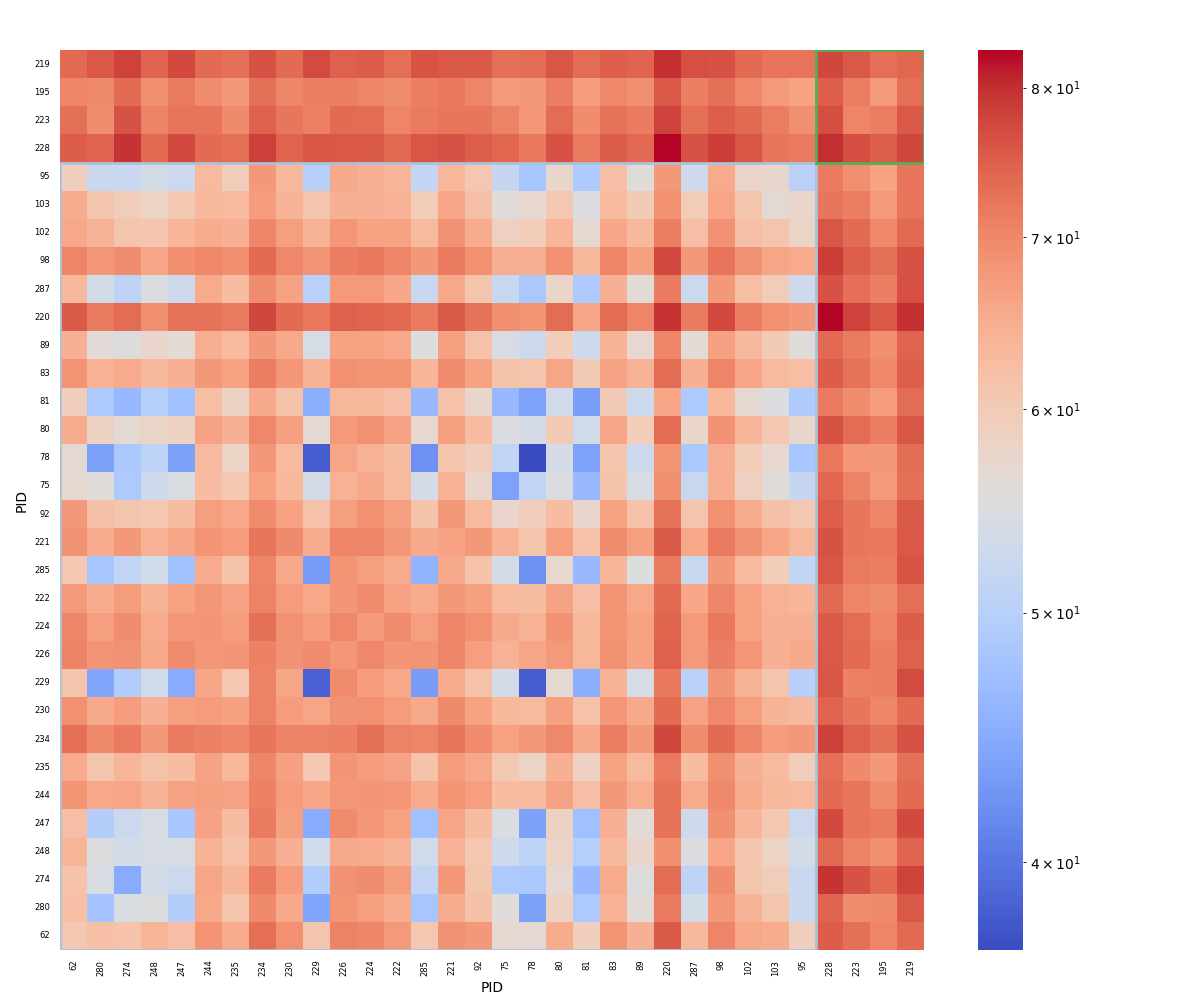
\includegraphics[width=\linewidth]{../plots/PID/DistanceMatrix.png}
	\caption{Matrix showing the similarity between participants taken from their mean euclidean distance measure shared with one and another. The matrix is sorted by proximity with the two clusters of participants outlined.}
	%	\figurenote{+10 gain represents the proportion who chose to lie for all amounts above 10 and also applies for +20 and +30.}
	\label{fig:DistanceMatrix}
\end{figure}

\subsubsection{Lie Percentage}

\begin{figure}[H]
	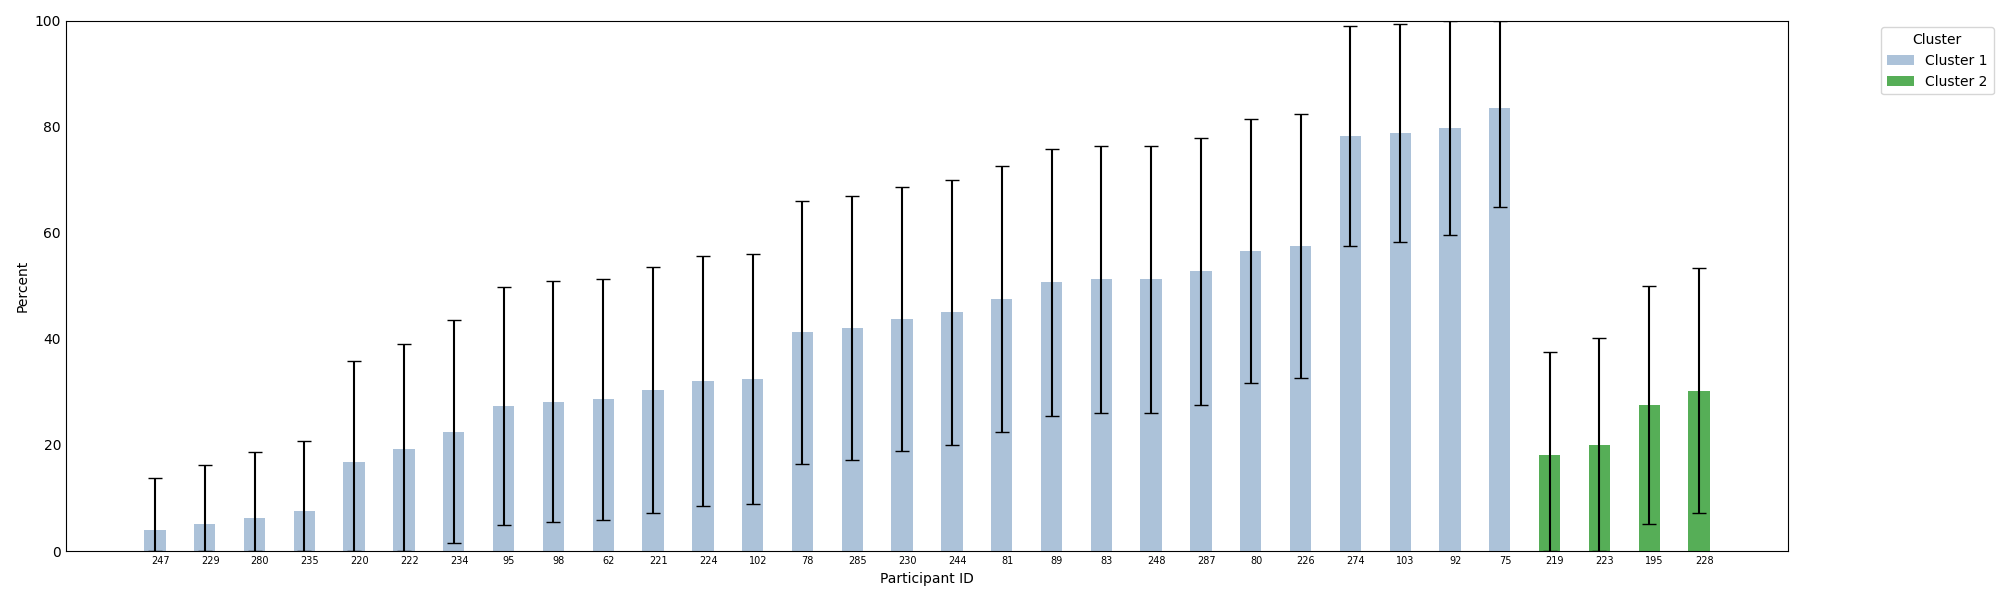
\includegraphics[width=\linewidth]{../plots/PID/PercentLiesByPID.png}
	\caption{Participants separated by hierarchical distance clustering and ordered by percentage lies.}
	%	\figurenote{+10 gain represents the proportion who chose to lie for all amounts above 10 and also applies for +20 and +30.}
	\label{fig:PercentLiesByPIDCluster}
\end{figure}

Using pairwise t-tests and calculating the mean statistic across clusters, it was deemed that the two clusters and their participant memberships showed to have a difference in lie percentage that was not significant $t(34)=1.6$, $p=.183$ (FDR corrected). Cluster 1 had a mean lie percentage of 37\% $(SD = 48\%)$ and cluster 2 had a mean of 42\% $(SD = 49)$. There was no significant difference within clusters either, for Cluster 1 $t(18)=1.1$, $p=.188$  and Cluster 2 $t(14)=1.4$, $p=.183$ (FDR corrected).

\subsubsection{Dwell Time}

 \begin{figure}[H]
 	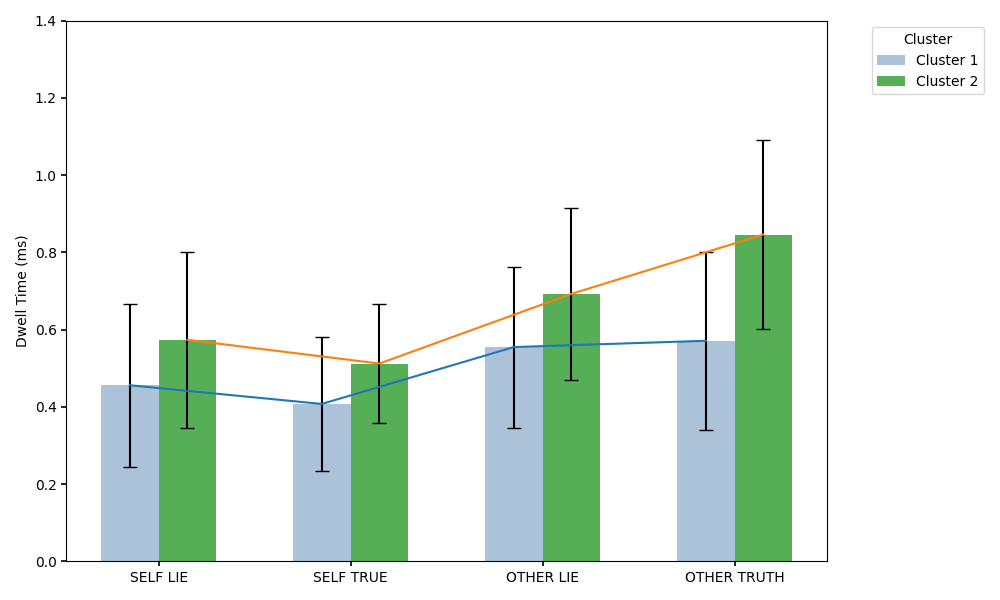
\includegraphics[width=\linewidth]{../plots/PID/DwellTimes.png}
 	\caption{Measures of average dwell time across participant clusters segmented by hierarchical distance clustering.}
 	%	\figurenote{+10 gain represents the proportion who chose to lie for all amounts above 10 and also applies for +20 and +30.}
 	\label{fig:DwellTimesByPIDCluster}
 \end{figure}

\begin{table}[H]
	\centering
	\begin{tabular}{|p{1.4cm}|p{1cm}|p{1cm}|p{1cm}|p{1cm}|p{1cm}|p{1cm}|p{1cm}|p{1cm}|p{1cm}|p{1cm}|}
		\hline
		\multirow{2}{*}{} & \multicolumn{4}{c|}{Cluster 1} & \multicolumn{4}{c|}{Cluster 2} & \multicolumn{2}{c|}{Between} \\ \cline{2-11}
		& $M$ (ms) &$SD$ (ms) & $t(20)$ & $p$ & $M$ (ms) & $SD$ (ms) & $t(18)$ & $p$ & $t(34)$ & $p$ \\ \hline
		\small{SELF LIE}& 0.49 & 0.38 & 0.17 & 0.215 & 0.24 & 0.34 & 1.5 & 0.14 & 1.9 & .126  \\ \hline
		\small{SELF TRUE} & 0.44 & 0.30 & 0.19 & 0.188 & 0.23 & 0.33 & 1.3 & 0.204 & 1.5 & .081  \\ \hline
		\small{OTHER LIE} & 0.51 & 0.32 & 0.12 & 0.239 & 0.39 & 0.49 & 1.1 & 0.159 & 0.19 & .211 \\ \hline
		\small{OTHER TRUTH} & 0.54 & 0.35 & -0.07 & 0.184 & 0.40 & 0.48 & -0.53 & 0.184& -0.15 & .184 \\ \hline
	\end{tabular}
	\vspace{0.3cm}
	\caption{Mean,. standard deviation and t tests for the average dwell time of each AOI across participant clusters. (FDR corrected)}
	\label{tab:NetLossDwellByPID}
\end{table}


In Table \ref{tab:NetLossDwellByPID}, average dwell times across the four AOIs show no significant differences when compared between and within clusters of participant membership.

\subsubsection{Number of Transitions}

 \begin{figure}[H]
	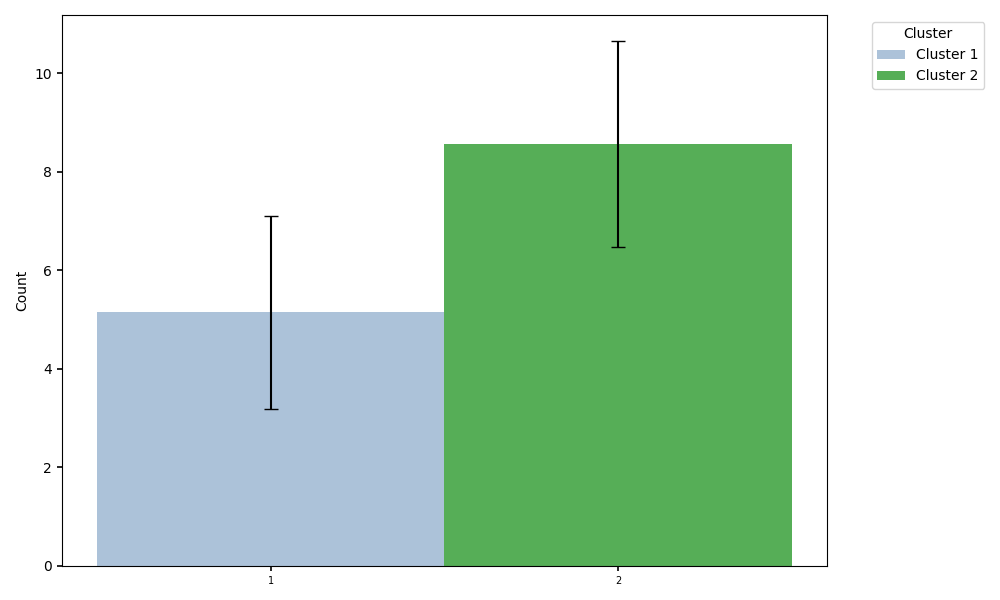
\includegraphics[width=\linewidth]{../plots/PID/NTransitions.png}
	\caption{Average number of transitions between clusters of participants determined from hierarchical clustering.}
	%	\figurenote{+10 gain represents the proportion who chose to lie for all amounts above 10 and also applies for +20 and +30.}
	\label{fig:NTransitionsByPIDCluster}
\end{figure}

The number of transitions averaged by the participants in Cluster 1 $(M = 9.2$, $SD = 4.6)$, showed to be significantly different to that of the participants in Cluster 2 $(M = 3.6\%$, $SD = 2.9\%)$, $t(34)=2.0$, $p=.042$. Comparatively, there was no significant difference in number of transitions within both Cluster 1 $t(34)=-0.75$, $p=.188$ and Cluster 2 $t(34)=1.5$, $p=.137$ (FDR corrected).

\subsection{Cross Analysis}

\subsubsection{Lie Percentage}

 \begin{figure}[H]
	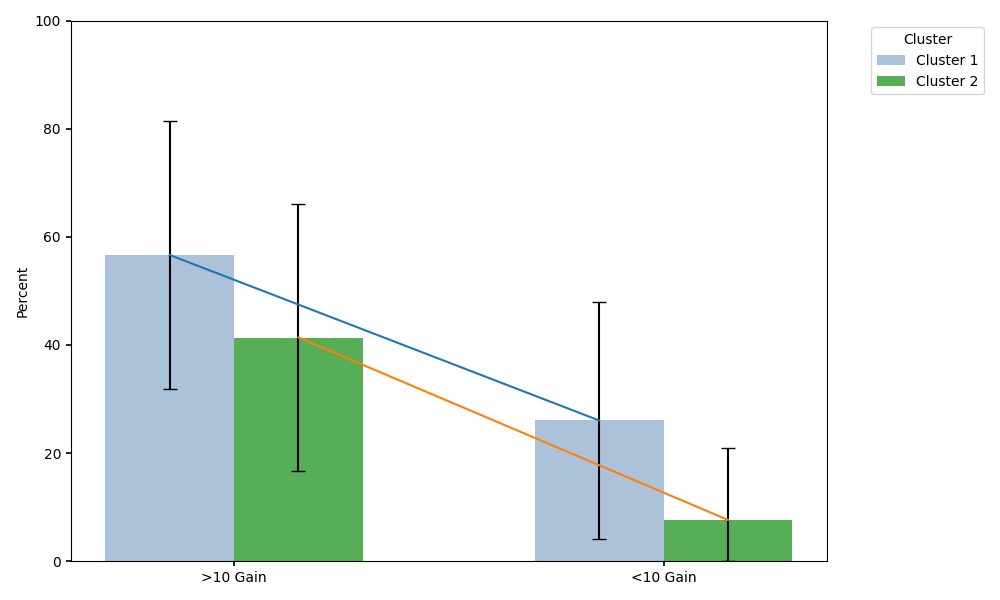
\includegraphics[width=\linewidth]{../plots/GainCluster/PercentLies.png}
	\caption{Average lie percentage for each cluster of participants across trial conditions dependent on net gain to sender.}
	%	\figurenote{+10 gain represents the proportion who chose to lie for all amounts above 10 and also applies for +20 and +30.}
	\label{fig:PercentLiesPerGainByPIDCluster}
\end{figure}

\begin{table}[H]
	\centering
	\begin{tabular}{|c|p{1.5cm}|p{2cm}|p{1.5cm}|p{2cm}|p{2cm}|p{1.5cm}|}
		\hline
		\multirow{2}{*}{} & \multicolumn{2}{c|}{<10 Gain to Sender} & \multicolumn{2}{c|}{>10 Gain to Sender} & \multicolumn{2}{c|}{T-test result} \\ \cline{2-7}
		& $M$ (\%) &$SD$ (\%) & $M$ (\%) & $SD$ (\%) & $t(66)$ & $p$ \\ \hline
		Cluster 1& 20 & 40 & 56 & 49 & -0.26 & .793  \\ \hline
		Cluster 2 & 34 & 47 & 52 & 50 & -0.74 & .460  \\ \hline
	\end{tabular}
	\vspace{0.3cm}
	\caption{Comparison of mean and standard deviation of average percent lie for each cluster across trial conditions (FDR Corrected)}
	\label{tab:PercentLiesPerGainByPIDCluster}
\end{table}



\subsubsection{Dwell Time}

 \begin{figure}[H]
	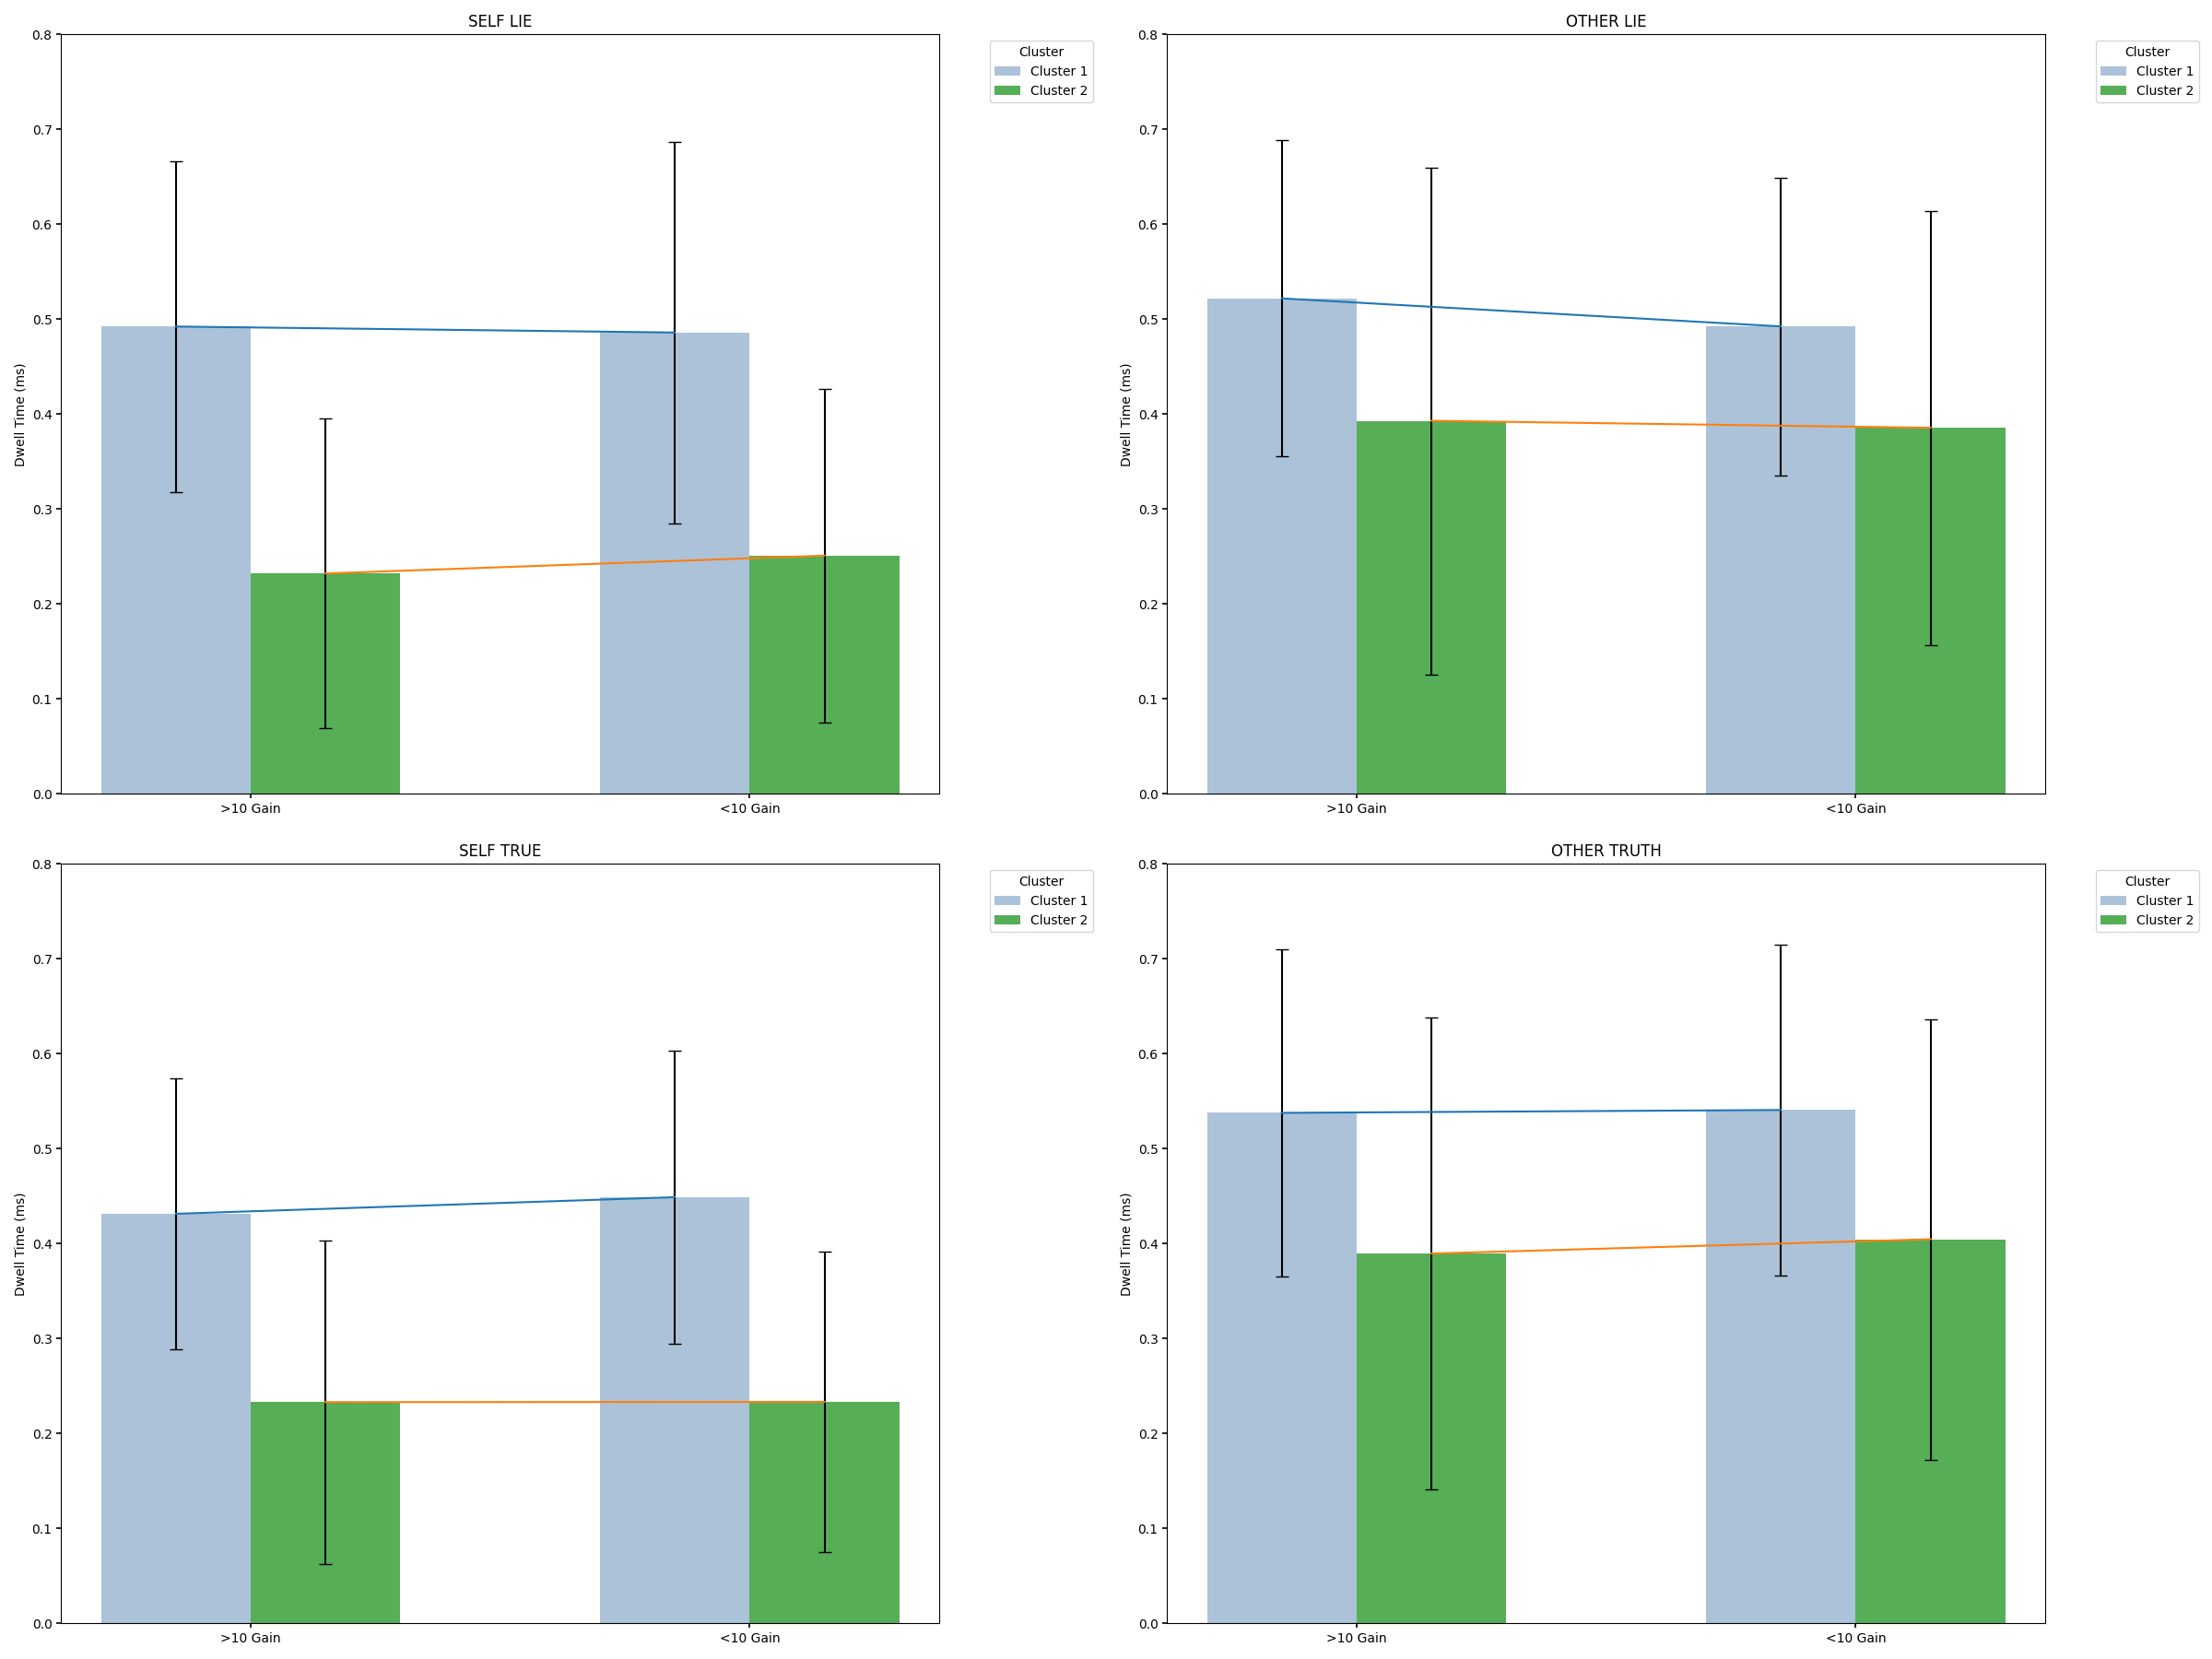
\includegraphics[width=\linewidth]{figures/GainClusterTiles.png}
	\caption{Measures of average dwell time across participant clusters segmented by hierarchical distance clustering.}
	%	\figurenote{+10 gain represents the proportion who chose to lie for all amounts above 10 and also applies for +20 and +30.}
	\label{fig:DwellTimesPerGainByPIDCluster}
\end{figure}

\begin{table}[H]
	\centering
	\begin{tabular}{|p{3.2cm}|p{0.7cm}|p{0.7cm}|p{0.7cm}|p{0.7cm}|p{0.9cm}|p{0.7cm}|p{0.7cm}|p{0.7cm}|p{0.8cm}|p{0.7cm}|}
		\hline
		\multirow{2}{*}{} & \multicolumn{4}{c|}{Gain to Sender < 10} & \multicolumn{4}{c|}{Gain to Sender > 10} & \multicolumn{2}{c|}{} \\ \cline{2-11}
		\multirow{2}{*}{} & \multicolumn{2}{c|}{Cluster 1} & \multicolumn{2}{c|}{Cluster 2} & \multicolumn{2}{c|}{Cluster 1} & \multicolumn{2}{c|}{Cluster 2} & \multicolumn{2}{c|}{T-test result} \\ \cline{2-11}
		& $M$ (ms) &$SD$ (ms) & $M$ (ms) & $SD$ (ms) & $M$ (ms) &$SD$ (ms) & $M$ (ms) & $SD$ (ms) & $t(34)$ & $p$ \\ \hline
		SELF LIE& 0.49 & 0.38 & 0.24 & 0.34 & 0.49 & 0.38 & 0.24 & 0.34 & 1.9 & .126  \\ \hline
		SELF TRUE & 0.44 & 0.30 & 0.23 & 0.33 & 0.49 & 0.38 & 0.24 & 0.34 & 1.5 & .081  \\ \hline
		OTHER LIE & 0.51 & 0.32 & 0.39 & 0.49 & 0.49 & 0.38 & 0.24 & 0.34 & 0.19 & .211 \\ \hline
		OTHER TRUTH & 0.54 & 0.35 & 0.40 & 0.48 & 0.49 & 0.38 & 0.24 & 0.34 & -0.15 & .184 \\ \hline
	\end{tabular}
	\vspace{0.3cm}
	\caption{Mean and standard deviation of the dwell time of each AOI across participant clusters. }
	\label{tab:NetGainDwellByPIDCluster}
\end{table}


\subsubsection{Number of Transitions}

 \begin{figure}[H]
	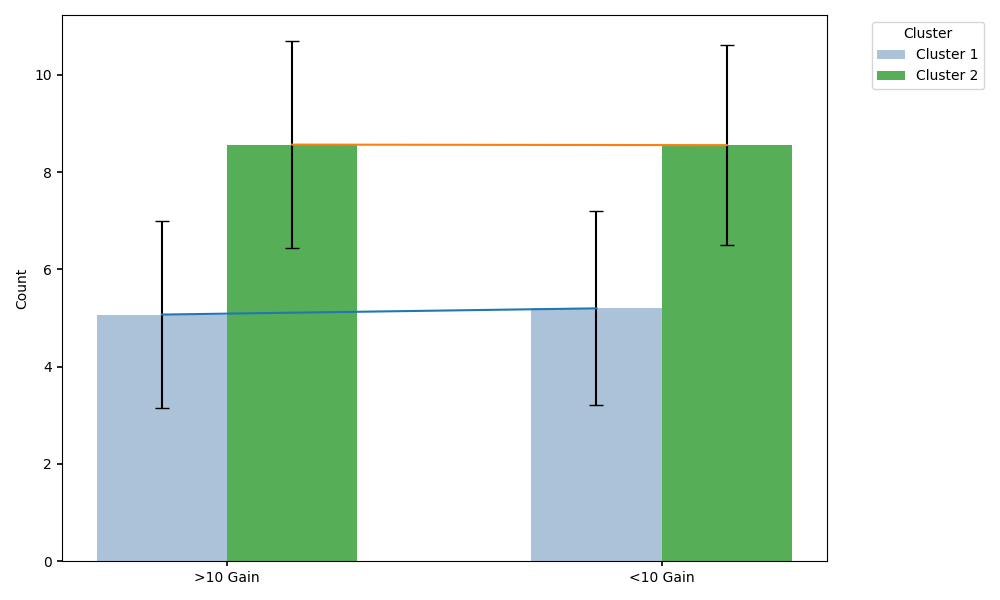
\includegraphics[width=\linewidth]{../plots/GainCluster/NTransitions.png}
	\caption{Measures of average dwell time across participant clusters segmented by hierarchical distance clustering.}
	%	\figurenote{+10 gain represents the proportion who chose to lie for all amounts above 10 and also applies for +20 and +30.}
	\label{fig:NTransitionPerGainByPIDCluster}
\end{figure}



%The analyses are presented in this section. These analyses may be quantitative or qualitative. Feel free to use as many graphs, tables and diagrams as you think necessary for presenting the analyses clearly.  Do not comment on the meaning of the results here. Extrapolating from your results will happen in your Discussion section


\section{Discussion}

% Discussion which includes: summary of results/findings, understanding of results/findings, critical perspective and insight, indication of future research, organization and structure, and clarity

%In this section, you will summarise your project, expand upon your results, offer insights into strengths and limitations of your study and/or future directions.

\printbibliography

% References which includes correct use of APA/BPS conventions

\appendix

%This section should contain details which are not essential to understanding the essence of the report. Lists of stimuli, tables of raw data, details of statistical analyses should be included here. The section must be neatly presented and clearly labelled. If you have a very large amount of data, such as might arise in qualitative studies you should consult with your supervisor about what should be included and how.

\end{document}